\documentclass{article}

% if you need to pass options to natbib, use, e.g.:
%     \PassOptionsToPackage{numbers, compress}{natbib}
% before loading neurips_2020



% to compile a preprint version, e.g., for submission to arXiv, add add the
% [preprint] option:
%     \usepackage[preprint]{neurips_2020}

% to compile a camera-ready version, add the [final] option, e.g.:
\usepackage[final, nonatbib]{neurips_2020}

% to avoid loading the natbib package, add option nonatbib:
     %\usepackage[nonatbib]{neurips_2020}

\usepackage[utf8]{inputenc} % allow utf-8 input
\usepackage[T1]{fontenc}    % use 8-bit T1 fonts
\usepackage{hyperref}       % hyperlinks
\usepackage{url}            % simple URL typesetting
\usepackage{booktabs}       % professional-quality tables
\usepackage{amsfonts}       % blackboard math symbols
\usepackage{nicefrac}       % compact symbols for 1/2, etc.
\usepackage{microtype}      % microtypography

% Our packages
\usepackage{graphicx}       % images
\usepackage{float}          % images
\usepackage{amsmath}        % math
\usepackage{bookmark}       % bookmarks
\usepackage[utf8]{inputenc} % accents

% Tighten spacing for figures
\setlength{\intextsep}{2pt}
\setlength{\textfloatsep}{2pt}
\setlength{\floatsep}{2pt}
\setlength{\abovecaptionskip}{2pt}
\setlength{\belowcaptionskip}{2pt}

% Tighten spacing for equations
\setlength{\abovedisplayskip}{0pt}
\setlength{\belowdisplayskip}{0pt}

\title{Behind the Face: Unveiling the Effects of Background Subtraction on VAE and GAN Model Efficacy}

% The \author macro works with any number of authors. There are two commands
% used to separate the names and addresses of multiple authors: \And and \AND.
%
% Using \And between authors leaves it to LaTeX to determine where to break the
% lines. Using \AND forces a line break at that point. So, if LaTeX puts 3 of 4
% authors names on the first line, and the last on the second line, try using
% \AND instead of \And before the third author name.

\author{%
  Thomas Kientz \\
  ENSAE Paris\\
  \texttt{thomas.kientz@ensae.fr} \\
  \And
  Elena Loumagne \\
  ENSAE Paris\\
  \texttt{elena.loumagne@ensae.fr} \\
  \AND
  Adèle Moreau \\
  ENSAE Paris\\
  \texttt{adele.moreau@ensae.fr} \\
}

\begin{document}

\maketitle

\begin{abstract}
  This study focuses on removing the background from datasets of faces to gauge the effect on the training and performance of facial generative models. We are also interested on the effect on the interpretability of the latent spaces of the models. 
\end{abstract}

The code for this project can be found on our repository \href{https://github.com/thomktz/FaceAI-BGImpact}{FaceAI-BGImpact}. \\
The demo video of the web-application we made can be watched \href{https://www.youtube.com/watch?v=BU1d8SxDASY}{here}.

\section{Introduction}

\quad The realm of image generation has seen some major breakthroughs in recent years. 
An area of specific interest to us was that of the latent representations of complex images in generative models. 
Observing these gives us an insight into what best characterizes an image, in the eyes of the trained algorithm. 
When applied to a dataset of human faces, they can give us objective\footnotemark insight into our most defining traits.
\footnotetext[1]{Depending on dataset bias}
Most image generation techniques will create an image from a scalar vector as input. 
During training, the algorithm will learn to map the dimensions of input vectors to different aspects of the image. 
This vector is what we are calling the latent vector, and its shape is the latent dimension. 
It can very well be interpreted as a compressed version of the image - indeed, a 128x128x3 RGB image is 49k+ scalars, and latent dimension is typically chosen to have 64-512 scalars. 

The key observation that we made was that in many trained face generation algorithms, the background of the image occupied a large portion\footnotemark of the captured variance - i.e. of the latent space. 
\footnotetext[2]{Metrics discussed later - PCA eigenvalues}
This means that some precious space from the latent vector is wasted on encoding what is behind the face, instead of the face itself. 

There are a few neutral-background datasets, but none of them have nearly enough samples to train generative algorithms, and are mostly used to train or fine tune classifiers. 
An index of such datasets can be found \href{https://libguides.princeton.edu/facedatabases}{here}. 
For image generation, we should aim for 10k-100k+ unique images, but none here exceed 1k with a neutral background.

\section{Related work}

\quad For the face generation task, some authors decided to circumvent the effect of the background by using a cropped version of their dataset to prevent various noisy backgrounds from interacting with the model \cite{gauthier2014conditional}. 

The impact of the background removal on Convolutional Neural Networks has been proved for classification tasks \cite{kcyin2021impact}. Achieving a 12\% higher accuracy on the task of Plant Disease Classification In-Situ for a dataset with images taken with a homogeneous background compared to that of a dataset with a cluttered background.

All these tricks suggest an important effect of the background on image generation. 
However, we have not found any studies on the importance of this effect of the background on image generation, and particularly face generation.

\section{Methodology}

\quad Our idea was to create our own neutral-background dataset, from a normal face dataset, \hyperlink{https://github.com/NVlabs/ffhq-dataset}{the Flicker-Faces-HQ dataset}, often used for facial generation tasks. 

To do this, we first decomposed the image by isolating the face and background using the \texttt{rembg} library. 
Then we created two datasets, one with a large Gaussian blur background and the other with a grey background. 
With over 70,000 images, our neutral background datasets are effective for training generative algorithms.

We focused on the 128x128 resolution version of the FFHQ dataset.
The datasets we generated were uploaded to Kaggle \hyperlink{https://www.kaggle.com/thomaskientz/datasets}{on this link}.

\textbf{Our main hypothesis is that the removal of the background will have a positive impact on the performance and the training of the generative models. 
Furthermore, we expect the latent space to be more interpretable.}

\begin{figure}[H]
    \centering
    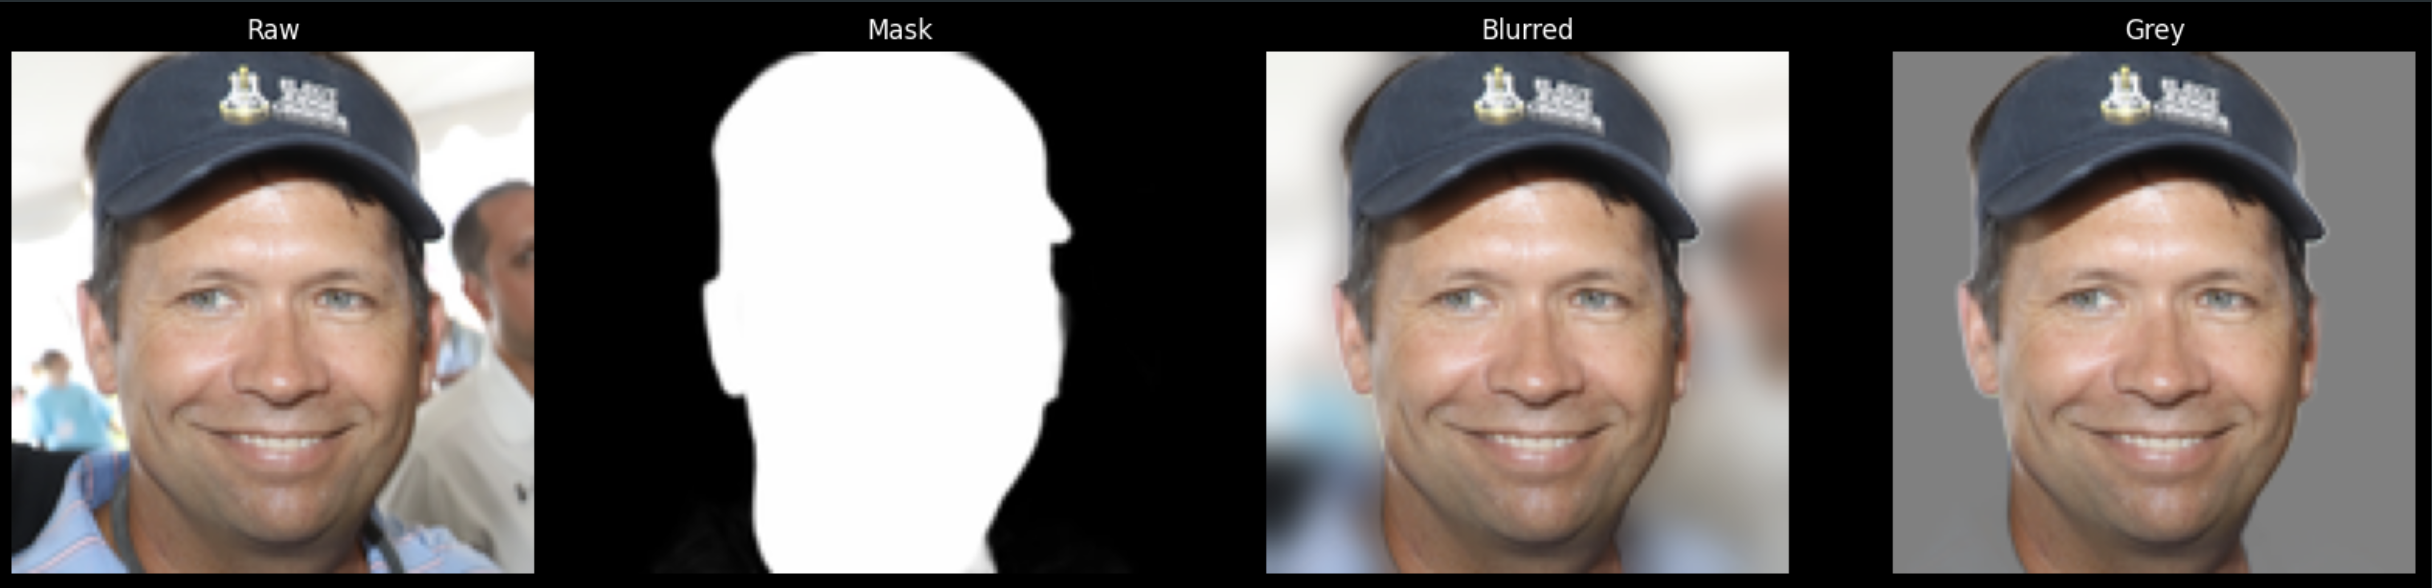
\includegraphics[width=0.8\textwidth]{images/mask.png}
    \caption{From left to right, original image, mask, blurred, greyed-out}
\end{figure}

To test our hypothesis, we trained models on both the original and the greyed-out versions of the same dataset. 
We picked versions of the two main categories of generative models: Auto-encoders (AE) and Generative Adversarial Networks (GAN).

\subsection{Auto-encoders}
\subsubsection*{Principle - Auto-encoders}

\quad Auto-encoders are unsupervised artificial neural networks whose main objective is to learn efficient representations of input data. 
An auto-encoder consists of two sub-networks: an encoder and a decoder. 
Firstly, the encoder compresses the input data (image) into a lower-dimensional representation. 
It reduces the dimensionality of the input data by mapping it to a set of hidden variables, often referred to as 'latent space'. 
The decoder then takes the encoded representation and reconstructs the original input data from it. 
The aim is to minimize the difference between the input and the reconstructed output, encouraging the model to learn a meaningful and compact representation.

\begin{figure}[H]
    \centering
    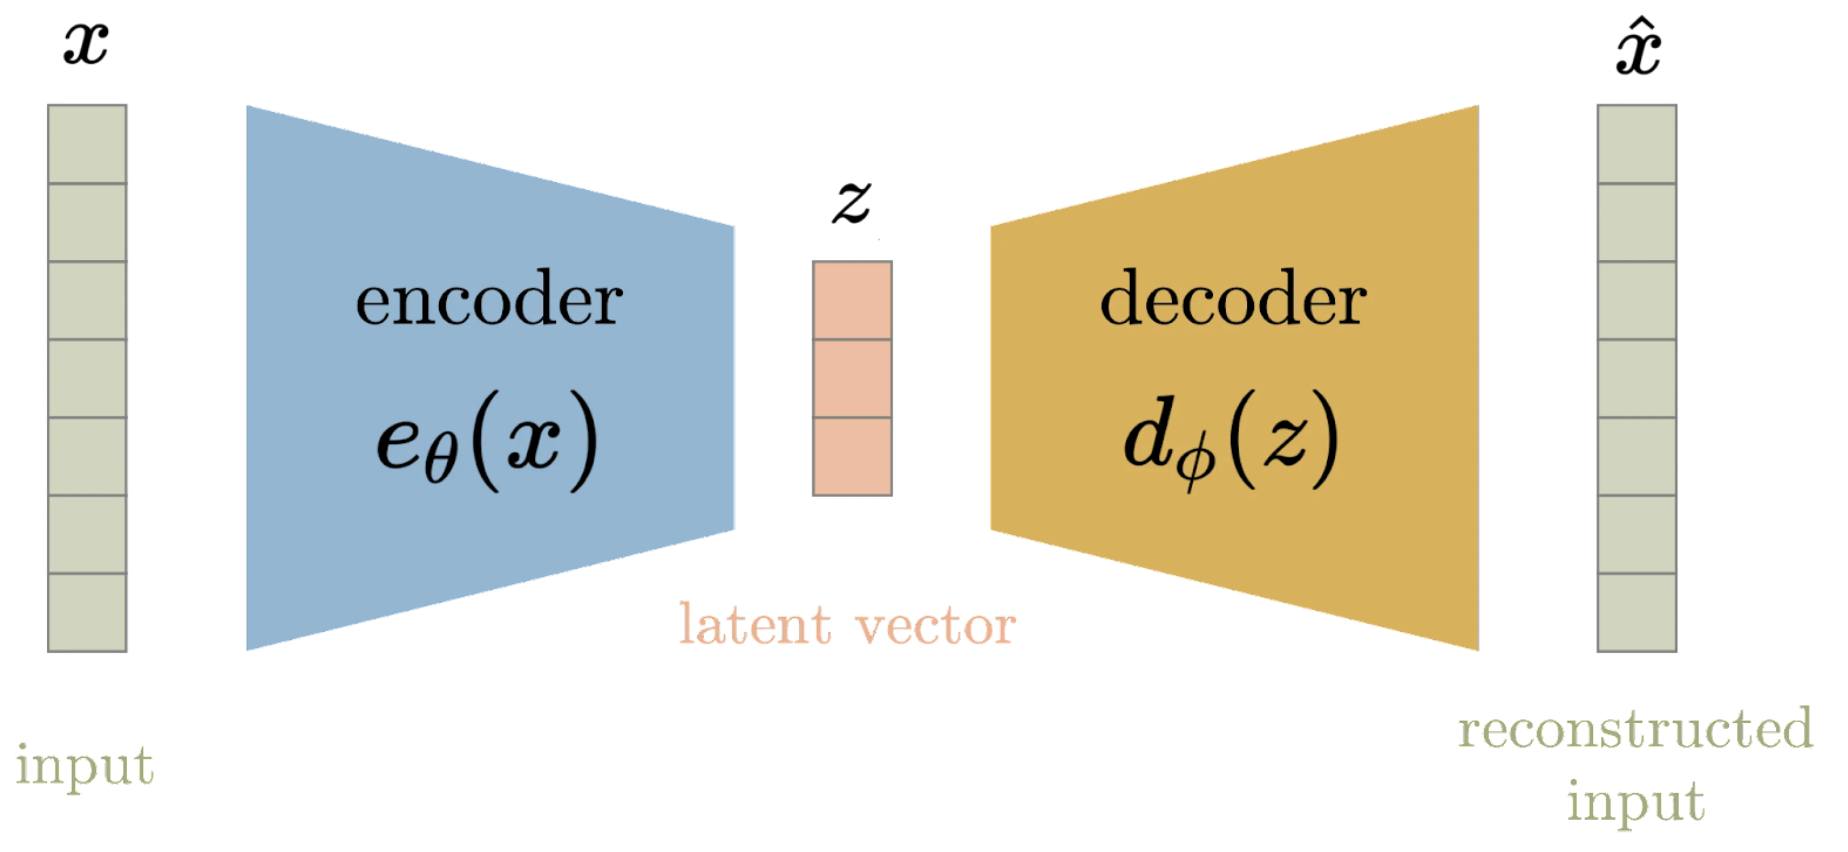
\includegraphics[width=0.6\textwidth]{images/ae.png}
    \caption{Auto-encoder architecture}
\end{figure}

Let $e_{\theta}:\mathcal{X}\to \mathcal{F}$ be the encoder function and $d_{\phi}:\mathcal{F}\to \mathcal{X}$ the decoder function. 
During training, input image $x$ is fed to the encoder function and passed through a series of layers that reduce their dimensions to give a compressed latent vector $z$. 
The number, type and size of the layers, as well as the size of the latent space, are parameters that can be controlled. 
Next, the decoder function maps the $\mathcal{F}$ latent space at the bottleneck to the output, attempting to recreate the original image after some generalized non-linear compression. 

The loss function used to train the neural network through the backpropagation procedure is as follows: 

\[\mathcal{L}(x,\hat{x})=\left\| x-\hat{x}\right\|_{2}=\left\| x-d_{\phi}(e_{\theta}(x)) \right\|_{2}\]

There is a trade-off between quality and latent dimensionality. Below a certain point, the latent space is too small to capture the important features of the input data, and all the images look the same.
This means that latent space of an auto-encoder also subject to irregularity due to overfitting. 

\subsubsection*{Principle - Variational Auto-encoders}
To tackle this problem, King et al. in 2013 \cite{kingma2013vae} proposed the Variational Auto-encoder (VAE) architecture. It addresses the problem of irregular latent space in a conventional auto-encoder by mapping inputs to parameters of a probability distribution instead of a fixed vector.
The VAE then imposes a constraint on this latent distribution, forcing it to be a Gaussian distribution, ensuring that the latent space is regularized.

\begin{figure}[H]
    \centering
    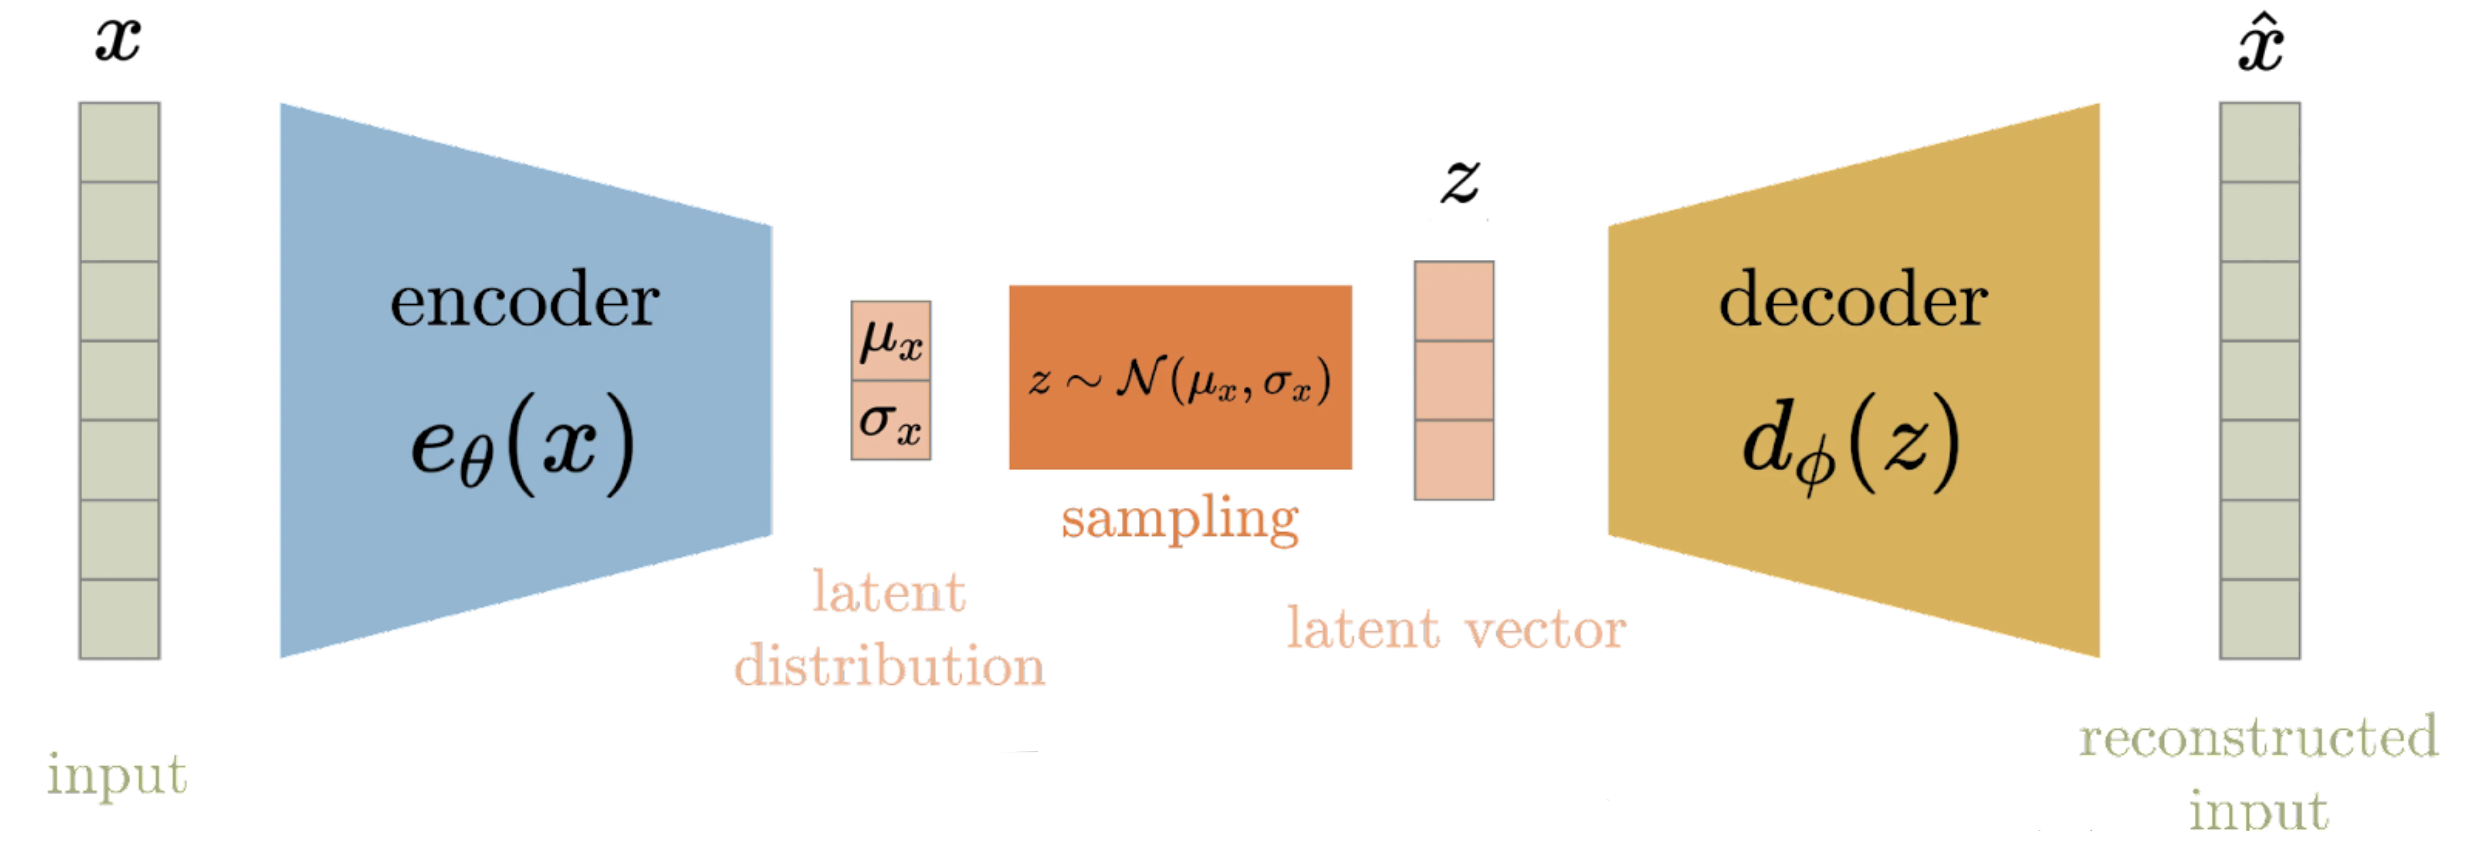
\includegraphics[width=0.8\textwidth]{images/vae.png}
    \caption{Variational Auto-encoder architecture}
\end{figure}

The VAE's encoder outputs the mean and standard deviation for each latent variable. The latent for the decoder is sampled from that distribution.

\subsubsection*{Rationale for choosing VAE}
VAEs generally perform better than regular AEs in image generation tasks. 
First, by learning a probabilistic latent space representation, it allows for smoother transitions and better interpolation in the latent space, which is crucial for generating diverse and realistic images. 
Then, VAEs inherently include a regularization term in their objective function, which encourages the learned latent space to be well-structured. 
This regularization helps prevent overfitting and aids in disentangling meaningful features in the latent space.
  
This is especially important for us, since we want to be able to interpret the latent space of our models.


\subsection{Generative Adversarial Networks}

\subsubsection*{Principle - Generative Adversarial Networks}

\quad Introduced by Ian Goodfellow and al. in 2014 \cite{goodfellow2014generative}, the Generative Adversarial Network consists of a Generator and a Discriminator, two neural networks that are trained simultaneously by adversarial training. \\
Firstly, the Generator model attempts to model the distribution of data in order to generate realistic samples. 
It takes as input a random noise sample of fixed size from a latent space and generates new false images. 
The main objective is to fool the Discriminator by transforming the random noise into images indistinguishable from the real ones, making it harder to classify images as true or false. 
Then, acting like a binary classifier, the Discriminator attempts to classify the input data as real or generated one. Training stops when the generated images look like real images.\\

In other words, the Generator and the Discriminator play a two-player minimax game : $\min_G \max_D V(D, G)$, where $\mathbf{z}$ is a random noise vector drawn from the latent space distribution, $D(\mathbf{x})$ the output of the discriminator and $G(\mathbf{z})$ is the output of the generator.\\

\subsubsection*{Principle - ProGANs}
One of the key features of the ProGAN architecture is the progressive nature of the layers, which enables the different visual characteristics of an image to be taken into account effectively. 
The concept is simple: the lower the layer and resolution, the greater the impact on coarser features. 
This granularity means that the inputs at each level can be modified independently, allowing precise control of the visual elements, from general characteristics to complex details, without affecting the other levels. 
The result is the generation of high-resolution images with a higher level of authenticity than previous models.


\begin{figure}[H]
    \centering
    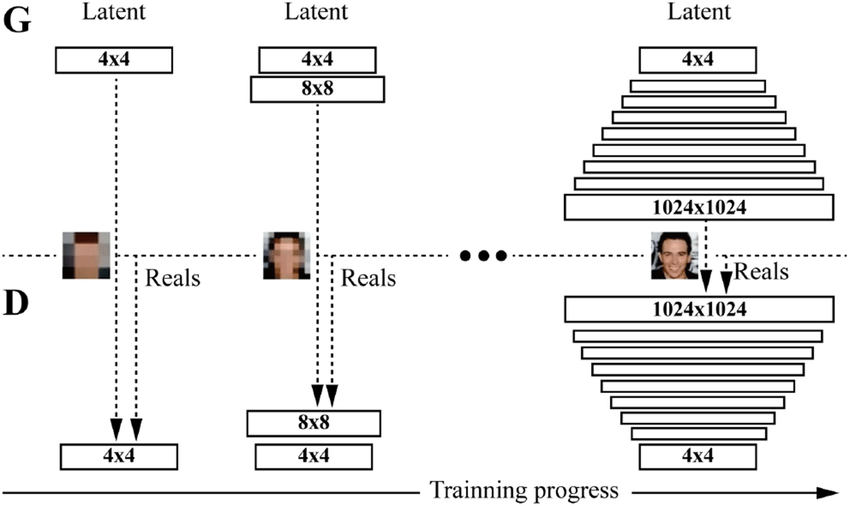
\includegraphics[width=0.5\textwidth]{images/progan.png}
    \caption{ProGAN training}
\end{figure}

In practice, the generator and discriminator are initialized with the full number of levels, but not all are used at first. Let's see the generation of an image at level 0 (i.e. at resolution 4x4):

\[\text{image}_{4x4}(z) = \text{ToRGB}_{4x4}(G_{4x4}(z))\]
\[\text{critic}_{4x4}(\text{image}) = D_{4x4}(\text{FromRGB}_{4x4}(\text{image}))\]

Now, at level 1 (resolution 8x8):

\[\text{image}_{8x8}(z) = \text{ToRGB}_{8x8}(G_{8x8}(G_{4x4}(z)))\]
\[\text{critic}_{8x8}(\text{image}) = D_{4x4}(D_{8x8}(\text{FromRGB}_{8x8}(\text{image})))\]

To prevent an explosion of gradients during the transition, we introduce $\alpha \in \left[0, 1\right]$, a parameter that controls the degree of blending between the two levels.

\[\text{image}_{8x8}(z, \alpha) = \alpha \times \text{image}_{8x8}(z) + (1-\alpha) \times Upscale(\text{image}_{4x4}(z))\]
\[\text{critic}_{8x8}(\text{image}, \alpha) = \alpha \times \text{critic}_{8x8}(\text{image}) + (1-\alpha) \times \text{critic}_{4x4}(DownScale(\text{image}))\]

The $\alpha$ parameter is increased linearly from 0 to 1 during the transition between levels 0 and 1. This process is repeated until the highest level is reached. 

ProGAN yields much better results than conventional GANs, but the latent space is still very disorganized and hard to interpret.

\subsubsection*{Principle - StyleGAN}

The main contribution of StyleGAN was to introduce a style-vector $w$ in the generator.

In each forward pass, a Mapping network $\mathcal{M}$ is used to map the latent vector $z$ to the intermediate latent space of styles, $w$.
Then, the generator $G$ uses $w$, instead of $z$, to generate the image. It also uses a learned constant $z_0$ to control the base style of the image, and some noise $\epsilon$.
\[w = \mathcal{M}(z)\]
\[\text{image}_{4x4}(w) = \text{ToRGB}_{4x4}(G_{4x4}(w, z_0, \epsilon))\]

The key difference is that in the level 1, 

\[\text{image}_{8x8}(w) = \text{ToRGB}_{8x8}(G_{8x8}(w, G_{4x4}(w, z_0, \epsilon), \epsilon))\]

The style vector $w$ is passed to the generator at each level.

\subsubsection*{Rationale for choosing StyleGAN}

The key features of StyleGAN over the other variants is that $w$ is supposedly more interpretable than $z$.

\subsubsection*{Training metric - FID}

\quad To evaluate the performance of our models, we used the Fréchet Inception Distance (FID) metric. Unlike other models, the losses of GANs are not very informative. The FID metric is a measure of the similarity between two datasets of images. 

The FID score is lower when the generated images closely match the real ones, indicating higher quality. 
The calculation involves two steps: feature extraction using the Inception model, a pre-trained deep learning model that extracts features and generates vector representations for each image. 
Then, the Fréchet Distance Calculation computes the mean and covariance of the feature vectors for both real and generated images, measuring the similarity between their distributions.

At resolution $l$ and blending factor $\alpha$, we're comparing blended real images $x(l, \alpha)$ and generated images $G_{l, \alpha}(w, z_0, \epsilon)$, with

\[ x(l, \alpha) = \alpha \times x_{l} + (1-\alpha) \times UpScale(x_{l-1}) \]

One think to keep in mind is that grey-background images weight 16\% less on average (raw 1.87Mb, grey 1.58Mb), because data was removed from them. We will be comparing what we define as an adjusted FID for the original dataset as follows:

\[ \text{FID}_{\text{adjusted}} = \text{FID}_{\text{raw}} \times (1 - 0.16) \]

Otherwise, the generation task is easier for the grey-background dataset, and the FID scores would be biased.

\section{Training}

\subsubsection*{Hardware setup}

These models require a lot of computing power. Luckily, in the end, a family member was able to provide us with SSH access into a Windows-Subsystems-for-Linux (WSL) environment within their computer. This computer had a NVIDIA GeForce RTX 3080 GPU.

\begin{table}[H]
  \centering
  \begin{tabular}{lcccccl}
    \toprule
    & \multicolumn{1}{c}{M1 CPU} & \multicolumn{1}{c}{Colab Free} & \multicolumn{1}{c}{Colab Pro} & \multicolumn{1}{c}{SSP Cloud\footnotemark} & \multicolumn{1}{c}{Family GPU} \\
    \midrule
    GPU & - & T4 & V100 & T4 & RTX 3080 \\
    Time per epoch\footnotemark (minutes) & 240 & 120 & 12 & 120 & 10 \\
    Cost per hour\footnotemark (cents€) & 0.8 & 0 & 45.8\footnotemark & 0 & 4 \\
    Cost per epoch (cents€) & 3.2 & 0 & 9.16 & 0 & 0.7 \\
    Cost for 400 epochs (€) & 12.8 & \textbf{0} & 36.6 & \textbf{0} & \textbf{2.8} \\
    Time for 400 epochs (hours) & 1600 & 800 & 80 & 800 & \textbf{66.7} \\
    \bottomrule
  \end{tabular}
  \caption{Time and Cost Analysis for the different GPU options - StyleGAN benchmark}
\end{table}

\footnotetext[1]{ENSAE provides us with an access to Datalab - SSP Cloud, with access to GPU instances}
\footnotetext[2]{Average over the different levels of StyleGAN - Resolution 4x4 is faster to train than 128x128.}
\footnotetext[3]{Taking into account electricity (M1 at 40W and RTX 3080 at 200W, at 0.20€/kWh).}
\footnotetext[4]{A Colab Pro subscription provides you with 100 compute units per month. These ran out in less than 24 hours of V100 training.}

The remote setup via SSH explains the large number of commits on the repository - we had to push our code to GitHub to be able to access it from the remote machine at each change we made.

\subsubsection*{VAE}

VAEs converge very quickly, and epochs are short (40s on our hardware). Below is a graph of the evolution of the FID during training.

\begin{figure}[H]
    \centering
    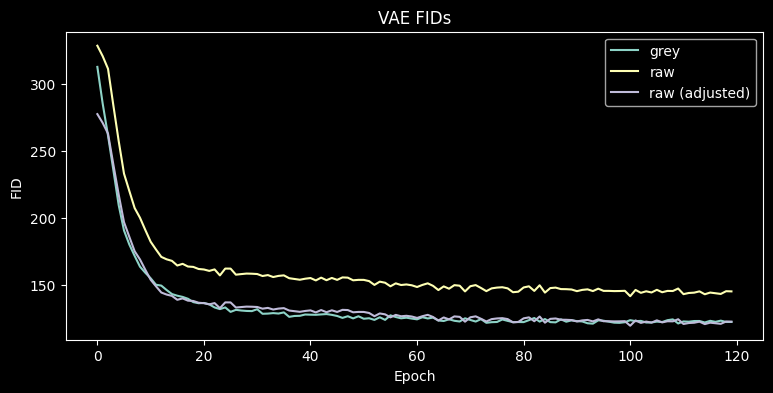
\includegraphics[width=0.7\textwidth]{images/vae_fids.png}
    \caption{Training of grey and original VAEs. "adjusted" refers to the weight adjustment.}
\end{figure}

We can conclude that both models converge to a comparable FID (in their own scale), at fairly high FID values. This is expected, as VAEs are not very good at generating realistic images. 

\subsubsection*{StyleGAN}
StyleGAN is a very ressource-intensive model. 
We trained each levels (i.e. resolution, starting from 4x4) until convergence of the FIDs. 

It is capital to ensure fairness in the training of the different datasets, for the results to be comparable. This means that they must train for the same number of epochs per level. To do so, we implemented a learning rate scheduler which slowly decreases the learning rate following an inverse sigmoid function during each level, and is reset at the beginning of the next level. This way, each model could train at appropriate learning rates during training.

Each level (=resolution) was trained sequentially, starting from 4x4 up to 128x128. Below are the FID scores for the 5th and final level (128x128).

\begin{figure}[H]
    \centering
    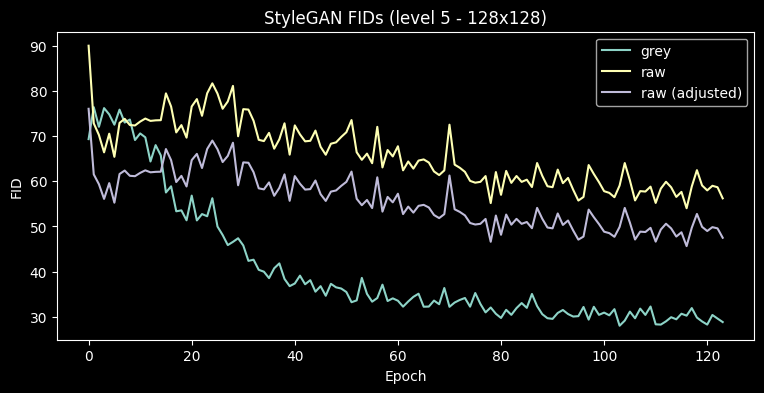
\includegraphics[width=0.7\textwidth]{images/stylegan_fids.png}
    \caption{Training of grey and original StyleGANs. "adjusted" refers to the weight adjustment.}
\end{figure}

Observations:
\begin{enumerate}
  \item \textbf{Even adjusted for image weight, the grey-background FIDs seems to converge faster and to a lower (better) value.}
  \item The FID levels are much lower than for the VAEs, which is expected.
\end{enumerate}

\section{Sample and control of the latent space}

Even with these models, sampling from the latent spaces is not straightforward.

\subsubsection*{VAE}

For each input image $x$, the encoder outputs $\mu_x, \sigma_x$. We can then sample $z$ from $\mathcal{N}(\mu_x, \sigma_x)$.
To generate now images, we can fit a Principal Component Analysis (PCA) on a large sample of $z$ generated from the true images to get the inverse transform $V_{\text{VAE}}$.
This allows us to sample and control the latent space using its eigenvectors in $z$ space:

\[z(x) = V_{\text{VAE}} \cdot x\]

This approach was inspired by CodeParade's video \href{https://www.youtube.com/watch?v=4VAkrUNLKSo}{"Computer Generates Human Faces"}, which introduced the idea of using PCA to control the latent space of a VAE.

\begin{figure}[H]
    \centering
    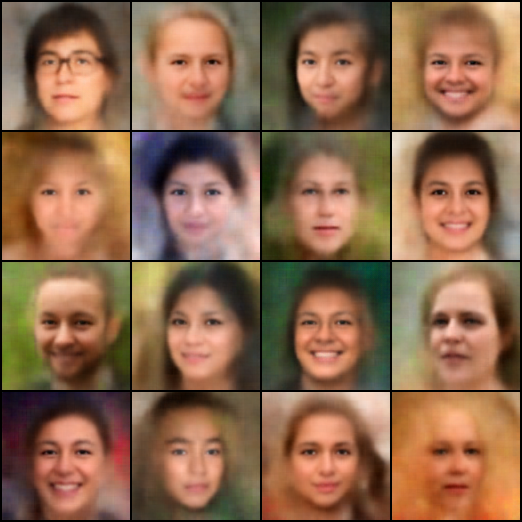
\includegraphics[width=0.32\textwidth]{images/sample_vae_raw.png}
    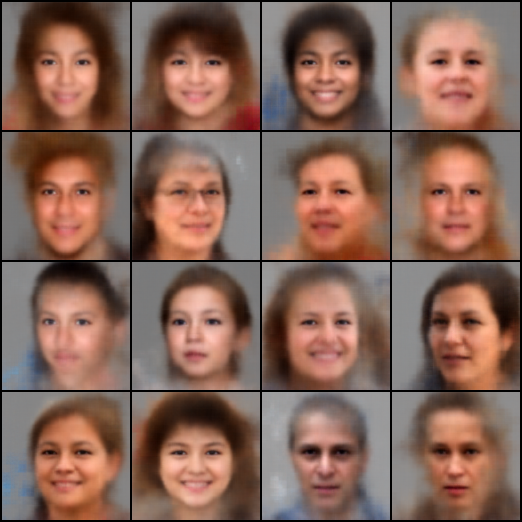
\includegraphics[width=0.32\textwidth]{images/sample_vae_grey.png}
    \caption{Samples from the raw and grey VAEs' latent spaces}
\end{figure}

It is hard to see any differences between the quality of the faces in the samples, which is expected given the equivalent adjusted FID scores.

\subsubsection*{StyleGAN}

For StyleGAN, we want to sample $w$ directly. For this, we will generate random $z$ and use the Mapping network $\mathcal{M}$ to map them to $w$.
We can then fit a PCA on a large sample of our synthetic $w$ to get the inverse transform $V_{\text{StyleGAN}}$.

\[w(x) = V_{\text{StyleGAN}} \cdot x\]

We also implemented style-blending, which is a technique where you can give different $w$ to different levels of the generator.
The GANSpace paper \cite{harkonen2020ganspace} was very helpful in understanding how to control the latent space of StyleGAN.

Here are samples from the latent space, $w$:

\begin{figure}[H]
  \centering
  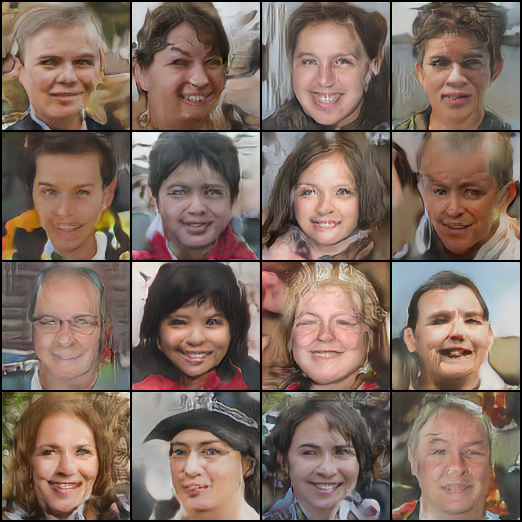
\includegraphics[width=0.32\textwidth]{images/sample_gan_raw.png}
  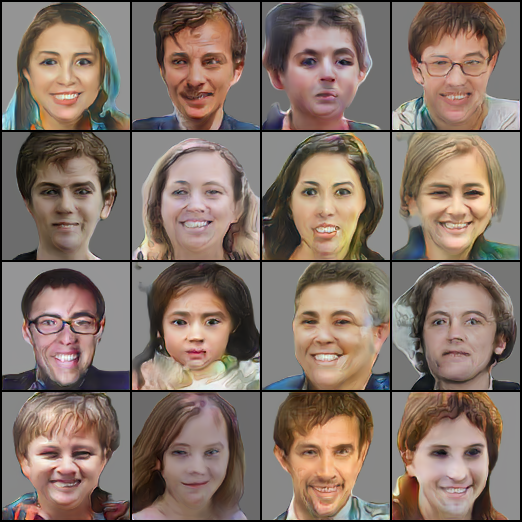
\includegraphics[width=0.32\textwidth]{images/sample_gan_grey.png}
  \caption{Samples from the raw and grey GANs' style latent spaces}
\end{figure}

Overall, these are much more detailed and diverse than the VAE samples, but introduce a lot of visual artefacts. 
The grey-background does seem to produce better quality images, as the FIDs would indicate, but that remains subjective.

Let's now compare the strongest eigenvectors of the PCA of the latent spaces. 
Each row below is the effect of varying the corresponding eigenvector from -3 to 3, leaving the others at 0. Each row $i$ represents the style vectors $(w_{i, t})_{t \in [0, 3]} = t \cdot \delta_i \cdot V_{\text{StyleGAN}}$, where $\delta_i$ is the Kronecker delta, and V is the PCA inverse transform.


\subsubsection*{Original (raw) - StyleGAN $w$ eigenvectors}


\begin{figure}[H]
  \centering
  \begin{minipage}{.18\linewidth}
      \centering
      $\lambda_{\text{raw}, 0} = 7.9$ \\
      BG brightness, hair
  \end{minipage}%
  \hfill
  \begin{minipage}{.81\linewidth}
      \centering
      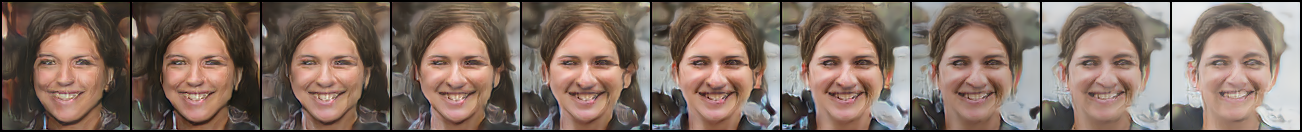
\includegraphics[width=\linewidth]{eigen/raw_gan_0.png}
  \end{minipage}
\end{figure}

\begin{figure}[H]
  \centering
  \begin{minipage}{.18\linewidth}
      \centering
      $\lambda_{\text{raw}, 1} = 5.8$ \\
      BG\footnotemark red-ness, head rotation
  \end{minipage}%
  \hfill
  \begin{minipage}{.81\linewidth}
      \centering
      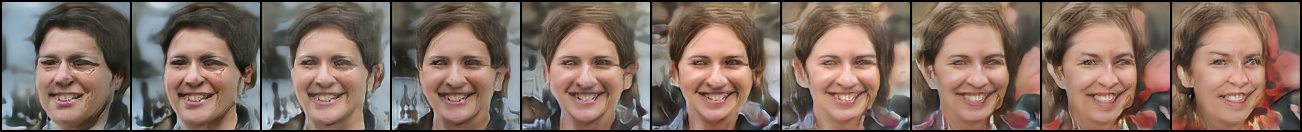
\includegraphics[width=\linewidth]{eigen/raw_gan_1.png}
  \end{minipage}
\end{figure}
\footnotetext[1]{Background}

\begin{figure}[H]
  \centering
  \begin{minipage}{.18\linewidth}
      \centering
      $\lambda_{\text{raw}, 2} = 5.2$ \\
      BG blue-ness, hair
  \end{minipage}%
  \hfill
  \begin{minipage}{.81\linewidth}
      \centering
      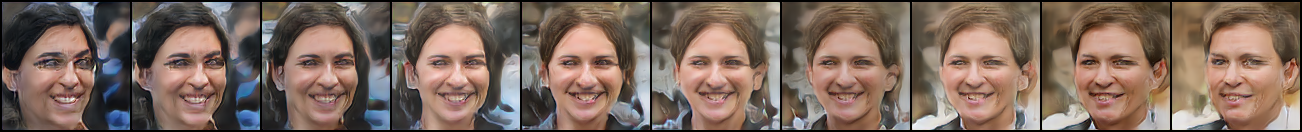
\includegraphics[width=\linewidth]{eigen/raw_gan_2.png}
  \end{minipage}
\end{figure}
  
\begin{figure}[H]
  \centering
  \begin{minipage}{.18\linewidth}
      \centering
      $\lambda_{\text{raw}, 3} = 4.8$ \\
      Glasses, gender, age
  \end{minipage}%
  \hfill
  \begin{minipage}{.81\linewidth}
      \centering
      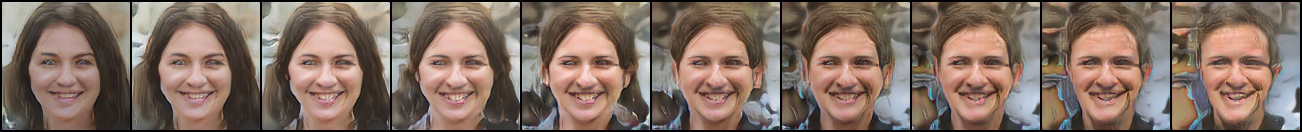
\includegraphics[width=\linewidth]{eigen/raw_gan_3.png}
  \end{minipage}
\end{figure}

\begin{figure}[H]
  \centering
  \begin{minipage}{.18\linewidth}
      \centering
      $\lambda_{\text{raw}, 4} = 4.4$ \\
      Glasses, gender, hair
  \end{minipage}%
  \hfill
  \begin{minipage}{.81\linewidth}
      \centering
      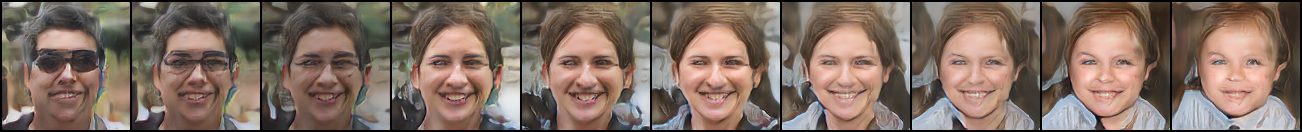
\includegraphics[width=\linewidth]{eigen/raw_gan_4.png}
  \end{minipage}
\end{figure}

The eigenvectors are very tangled with background variations, and the effects on the facial features themselves are not big.

\subsubsection*{Grey-background - StyleGAN $w$ eigenvectors}

\begin{figure}[H]
  \centering
  \begin{minipage}{.18\linewidth}
      \centering
      $\lambda_{\text{grey, 0}} = 4.3$ \\
      Gender, hair
  \end{minipage}%
  \hfill
  \begin{minipage}{.81\linewidth}
      \centering
      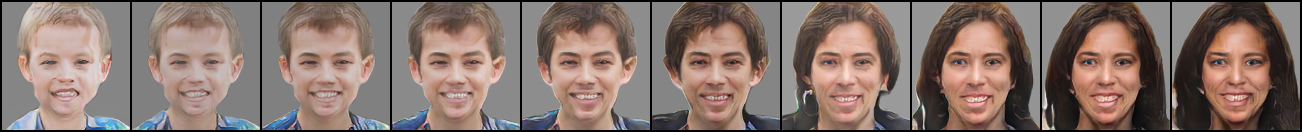
\includegraphics[width=\linewidth]{eigen/grey_gan_0.png}
  \end{minipage}
\end{figure}

\begin{figure}[H]
  \centering
  \begin{minipage}{.18\linewidth}
      \centering
      $\lambda_{\text{grey, 1}} = 3.1$ \\
      Gender, lipstick, hair
  \end{minipage}%
  \hfill
  \begin{minipage}{.81\linewidth}
      \centering
      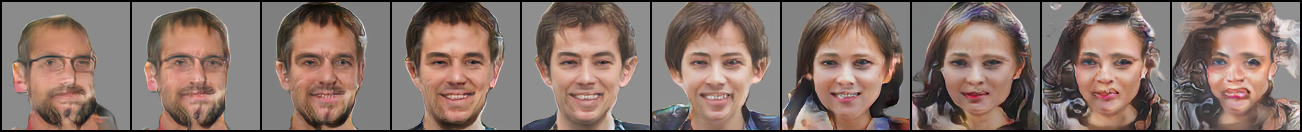
\includegraphics[width=\linewidth]{eigen/grey_gan_1.png}
  \end{minipage}
\end{figure}

\begin{figure}[H]
  \centering
  \begin{minipage}{.18\linewidth}
      \centering
      $\lambda_{\text{grey, 2}} = 2.5$ \\
      Head rotation
  \end{minipage}%
  \hfill
  \begin{minipage}{.81\linewidth}
      \centering
      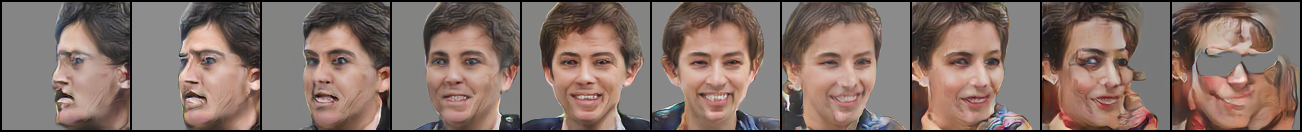
\includegraphics[width=\linewidth]{eigen/grey_gan_2.png}
  \end{minipage}
\end{figure}
  
\begin{figure}[H]
  \centering
  \begin{minipage}{.18\linewidth}
      \centering
      $\lambda_{\text{grey, 3}} = 2.2$ \\
      Gender, skin, hair
  \end{minipage}%
  \hfill
  \begin{minipage}{.81\linewidth}
      \centering
      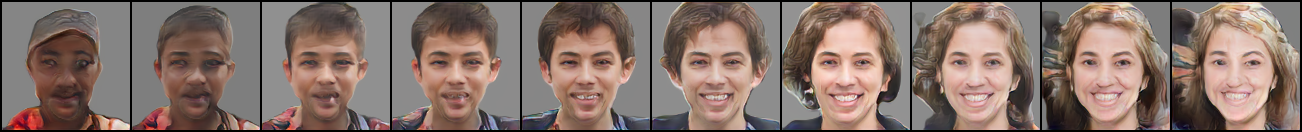
\includegraphics[width=\linewidth]{eigen/grey_gan_3.png}
  \end{minipage}
\end{figure}

\begin{figure}[H]
  \centering
  \begin{minipage}{.18\linewidth}
      \centering
      $\lambda_{\text{grey, 4}} = 1.9$ \\
      Glasses, gender, hair
  \end{minipage}%
  \hfill
  \begin{minipage}{.81\linewidth}
      \centering
      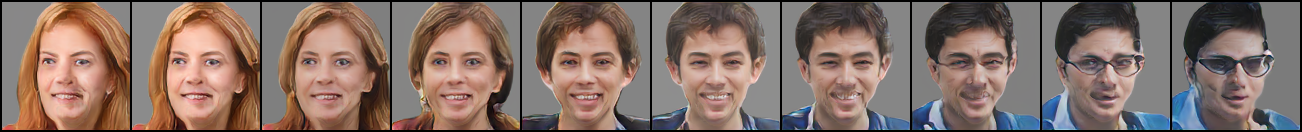
\includegraphics[width=\linewidth]{eigen/grey_gan_4.png}
  \end{minipage}
\end{figure}

The grey-background eigenvectors seem to have a much more pronounced and clear effect on the facial attributes, even though the eigenvalues are smaller. \\
\textbf{This demonstrates that a lot of the variance is uselessly captured by the background in the original model, and shows the effectiveness of our method at tackling this problem.}\\
This is clear when comparing $\lambda_{\text{raw}, 1}$ and $\lambda_{\text{grey, 2}}$, two eigenvectors that capture head rotation.

The same can be observed in the VAE eigenvectors:

\subsubsection*{Original (raw) - VAE $z$ eigenvectors}

\begin{figure}[H]
  \centering
  \begin{minipage}{.18\linewidth}
      \centering
      $\lambda_{\text{raw}, 0} = 1.19$ \\
      BG color
  \end{minipage}%
  \hfill
  \begin{minipage}{.81\linewidth}
      \centering
      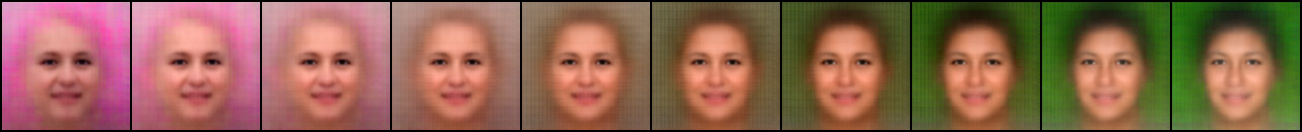
\includegraphics[width=\linewidth]{eigen/raw_vae_0.png}
  \end{minipage}
\end{figure}

\subsubsection*{Grey-background - VAE $z$ eigenvectors}

\begin{figure}[H]
  \centering
  \begin{minipage}{.18\linewidth}
      \centering
      $\lambda_{\text{grey}, 0} = 1.18$ \\
      Hair, head rotation
  \end{minipage}%
  \hfill
  \begin{minipage}{.81\linewidth}
      \centering
      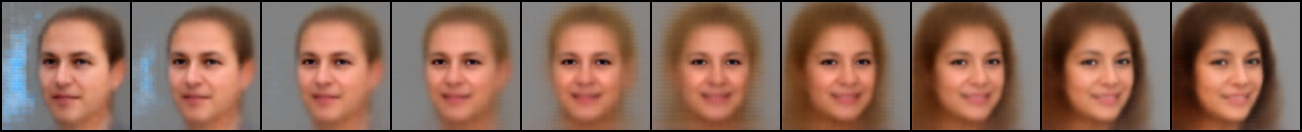
\includegraphics[width=\linewidth]{eigen/grey_vae_0.png}
  \end{minipage}
\end{figure}


A full list of the eigenvectors can be found in the Appendix.

\newpage
\bibliographystyle{plain}  % Choose a style that suits your needs
\bibliography{bibtex}  % The filename of your .bib file (without extension)

\newpage
\section*{Appendix}

\subsubsection*{Grey-background - StyleGAN $w$ eigenvectors 0-14}

\begin{figure}[H]
  \centering
  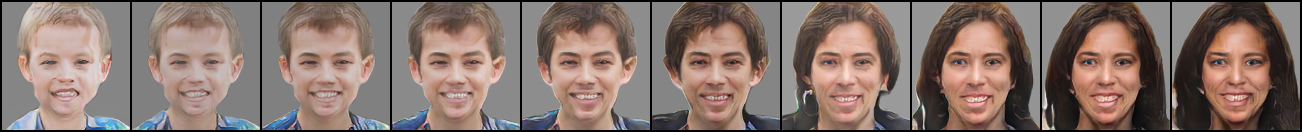
\includegraphics[width=0.9\linewidth]{eigen/grey_gan_0.png}
  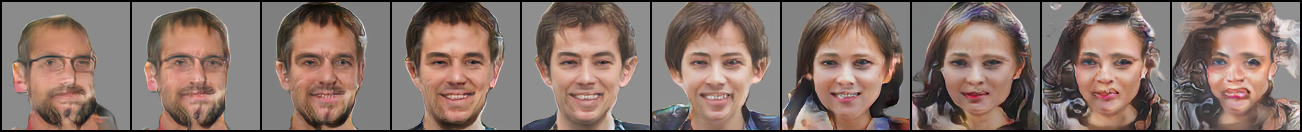
\includegraphics[width=0.9\linewidth]{eigen/grey_gan_1.png}
  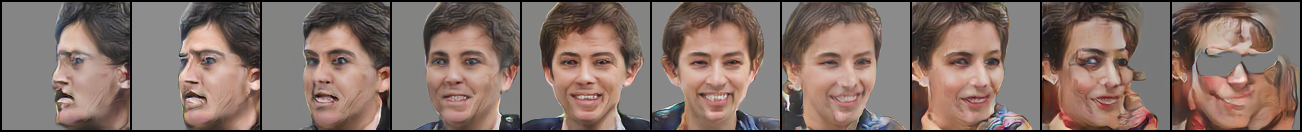
\includegraphics[width=0.9\linewidth]{eigen/grey_gan_2.png}
  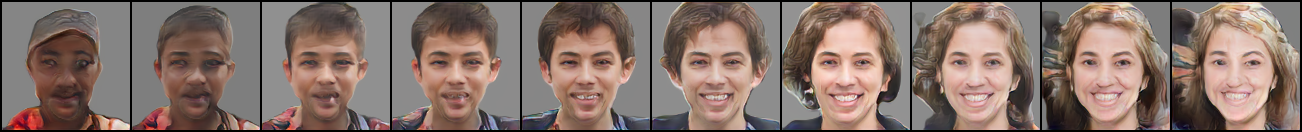
\includegraphics[width=0.9\linewidth]{eigen/grey_gan_3.png}
  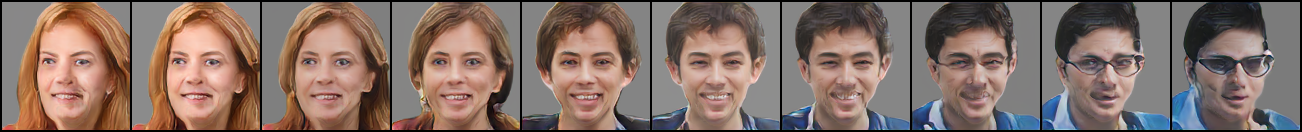
\includegraphics[width=0.9\linewidth]{eigen/grey_gan_4.png}
  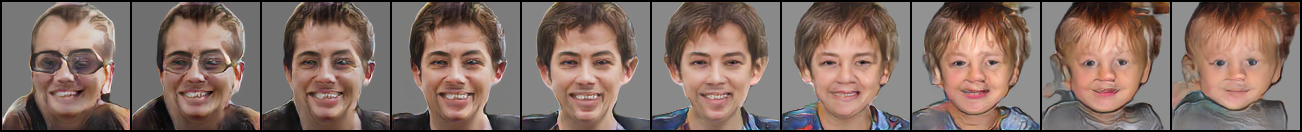
\includegraphics[width=0.9\linewidth]{eigen/grey_gan_5.png}
  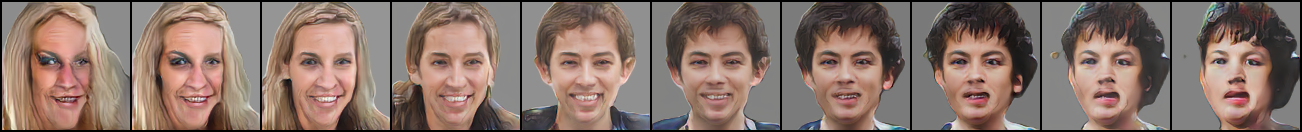
\includegraphics[width=0.9\linewidth]{eigen/grey_gan_6.png}
  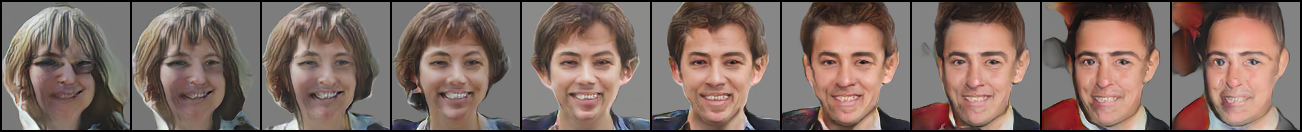
\includegraphics[width=0.9\linewidth]{eigen/grey_gan_7.png}
  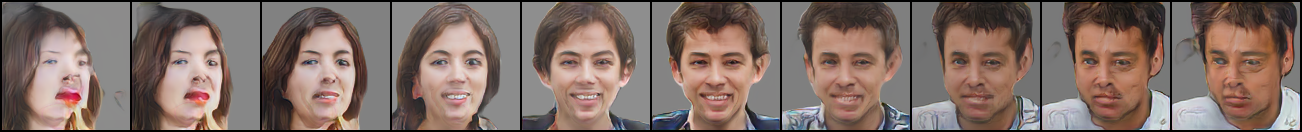
\includegraphics[width=0.9\linewidth]{eigen/grey_gan_8.png}
  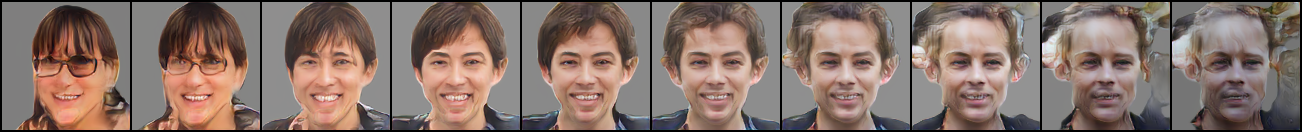
\includegraphics[width=0.9\linewidth]{eigen/grey_gan_9.png}
  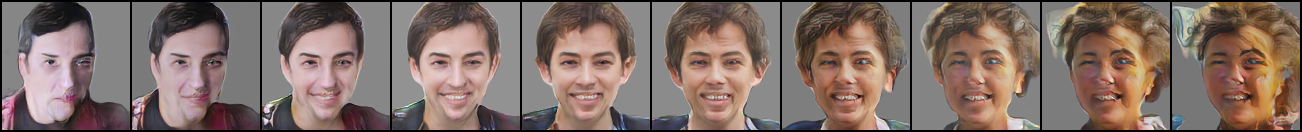
\includegraphics[width=0.9\linewidth]{eigen/grey_gan_10.png}
  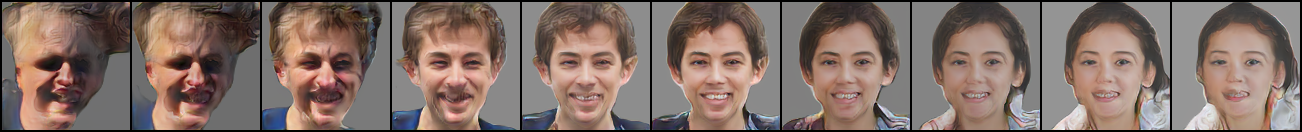
\includegraphics[width=0.9\linewidth]{eigen/grey_gan_11.png}
  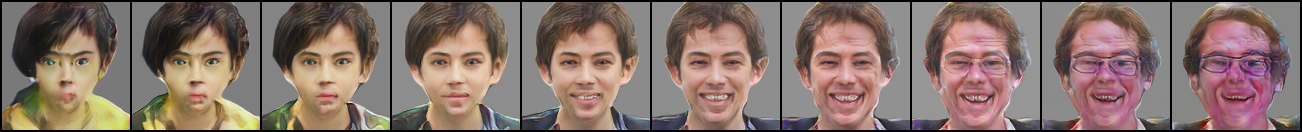
\includegraphics[width=0.9\linewidth]{eigen/grey_gan_12.png}
  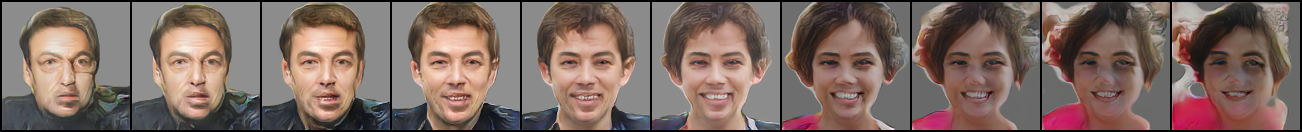
\includegraphics[width=0.9\linewidth]{eigen/grey_gan_13.png}
  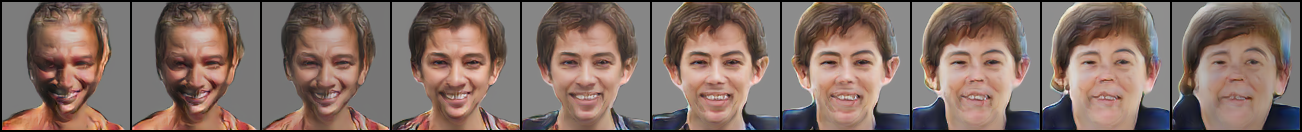
\includegraphics[width=0.9\linewidth]{eigen/grey_gan_14.png}
\end{figure}

\newpage
\subsubsection*{Grey-background - StyleGAN $w$ eigenvectors 15-29}

\begin{figure}[H]
  \centering
  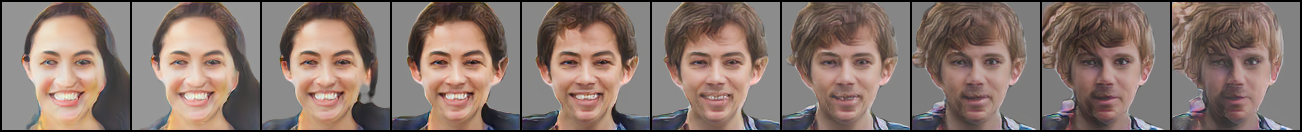
\includegraphics[width=0.9\linewidth]{eigen/grey_gan_15.png}
  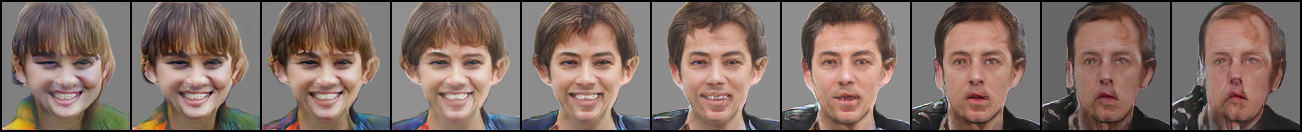
\includegraphics[width=0.9\linewidth]{eigen/grey_gan_16.png}
  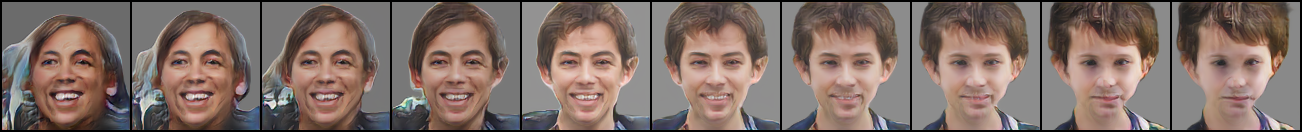
\includegraphics[width=0.9\linewidth]{eigen/grey_gan_17.png}
  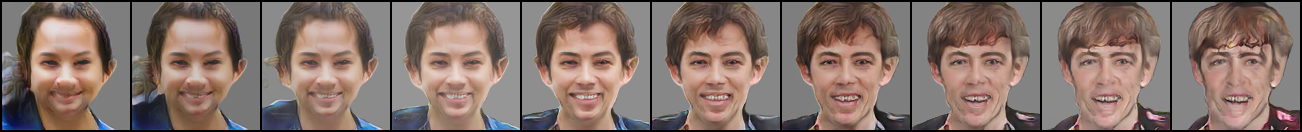
\includegraphics[width=0.9\linewidth]{eigen/grey_gan_18.png}
  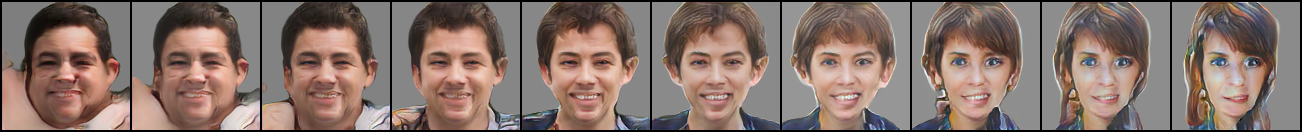
\includegraphics[width=0.9\linewidth]{eigen/grey_gan_19.png}
  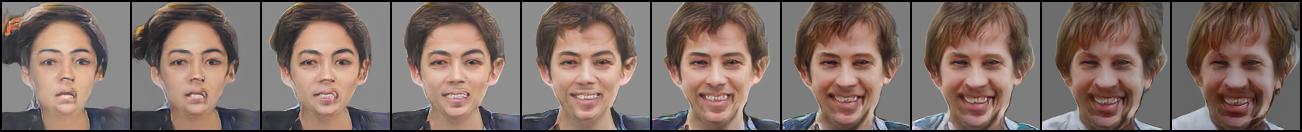
\includegraphics[width=0.9\linewidth]{eigen/grey_gan_20.png}
  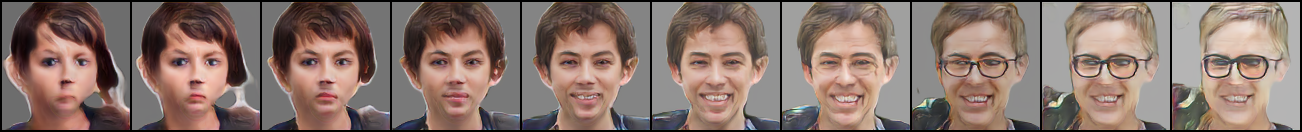
\includegraphics[width=0.9\linewidth]{eigen/grey_gan_21.png}
  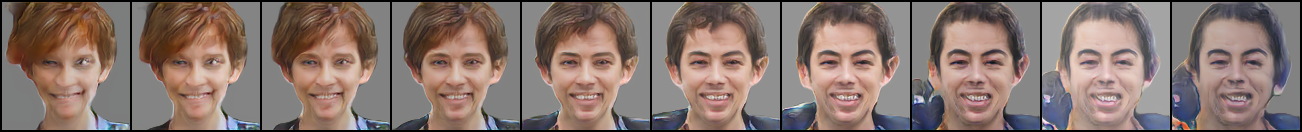
\includegraphics[width=0.9\linewidth]{eigen/grey_gan_22.png}
  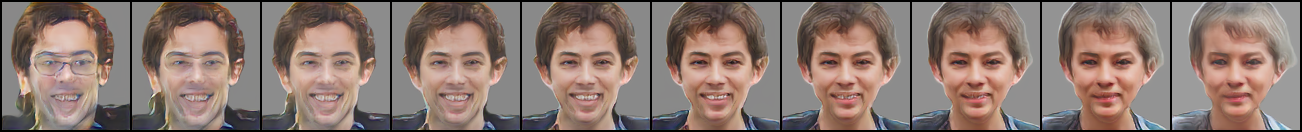
\includegraphics[width=0.9\linewidth]{eigen/grey_gan_23.png}
  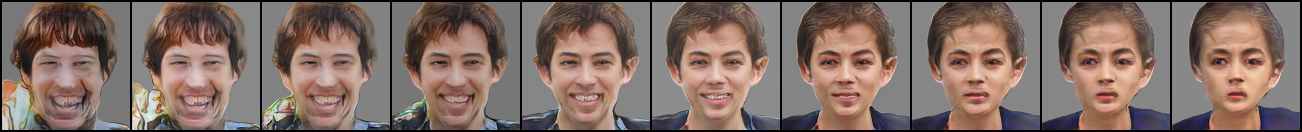
\includegraphics[width=0.9\linewidth]{eigen/grey_gan_24.png}
  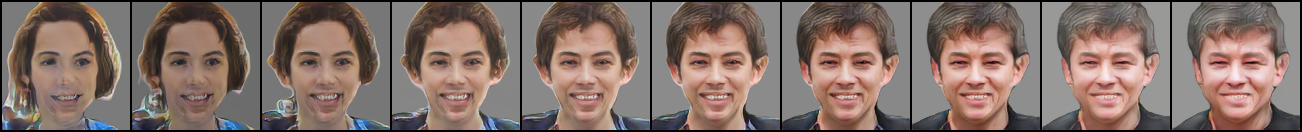
\includegraphics[width=0.9\linewidth]{eigen/grey_gan_25.png}
  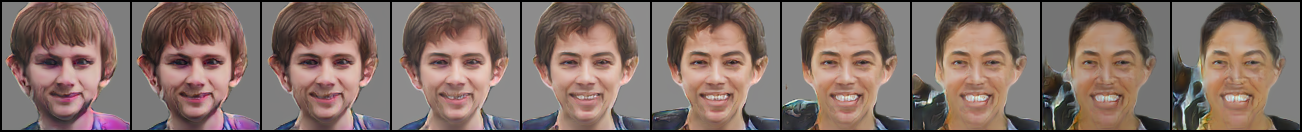
\includegraphics[width=0.9\linewidth]{eigen/grey_gan_26.png}
  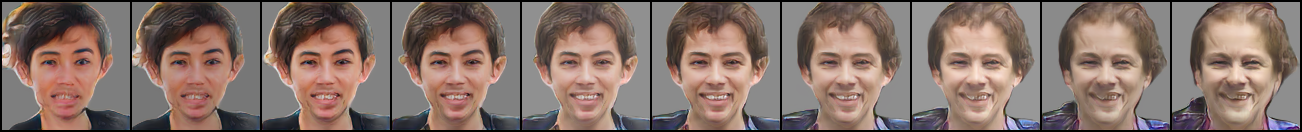
\includegraphics[width=0.9\linewidth]{eigen/grey_gan_27.png}
  \includegraphics[width=0.9\linewidth]{eigen/grey_gan_28.png}
  \includegraphics[width=0.9\linewidth]{eigen/grey_gan_29.png}

\end{figure}
\newpage

\subsubsection*{Original (raw) - StyleGAN $w$ eigenvectors 0-14}

\begin{figure}[H]
  \centering
  \includegraphics[width=0.9\linewidth]{eigen/raw_gan_0.png}
  \includegraphics[width=0.9\linewidth]{eigen/raw_gan_1.png}
  \includegraphics[width=0.9\linewidth]{eigen/raw_gan_2.png}
  \includegraphics[width=0.9\linewidth]{eigen/raw_gan_3.png}
  \includegraphics[width=0.9\linewidth]{eigen/raw_gan_4.png}
  \includegraphics[width=0.9\linewidth]{eigen/raw_gan_5.png}
  \includegraphics[width=0.9\linewidth]{eigen/raw_gan_6.png}
  \includegraphics[width=0.9\linewidth]{eigen/raw_gan_7.png}
  \includegraphics[width=0.9\linewidth]{eigen/raw_gan_8.png}
  \includegraphics[width=0.9\linewidth]{eigen/raw_gan_9.png}
  \includegraphics[width=0.9\linewidth]{eigen/raw_gan_10.png}
  \includegraphics[width=0.9\linewidth]{eigen/raw_gan_11.png}
  \includegraphics[width=0.9\linewidth]{eigen/raw_gan_12.png}
  \includegraphics[width=0.9\linewidth]{eigen/raw_gan_13.png}
  \includegraphics[width=0.9\linewidth]{eigen/raw_gan_14.png}
\end{figure}

\newpage
\subsubsection*{Original (raw) - StyleGAN $w$ eigenvectors 15-29}

\begin{figure}[H]
  \centering
  \includegraphics[width=0.9\linewidth]{eigen/raw_gan_15.png}
  \includegraphics[width=0.9\linewidth]{eigen/raw_gan_16.png}
  \includegraphics[width=0.9\linewidth]{eigen/raw_gan_17.png}
  \includegraphics[width=0.9\linewidth]{eigen/raw_gan_18.png}
  \includegraphics[width=0.9\linewidth]{eigen/raw_gan_19.png}
  \includegraphics[width=0.9\linewidth]{eigen/raw_gan_20.png}
  \includegraphics[width=0.9\linewidth]{eigen/raw_gan_21.png}
  \includegraphics[width=0.9\linewidth]{eigen/raw_gan_22.png}
  \includegraphics[width=0.9\linewidth]{eigen/raw_gan_23.png}
  \includegraphics[width=0.9\linewidth]{eigen/raw_gan_24.png}
  \includegraphics[width=0.9\linewidth]{eigen/raw_gan_25.png}
  \includegraphics[width=0.9\linewidth]{eigen/raw_gan_26.png}
  \includegraphics[width=0.9\linewidth]{eigen/raw_gan_27.png}
  \includegraphics[width=0.9\linewidth]{eigen/raw_gan_28.png}
  \includegraphics[width=0.9\linewidth]{eigen/raw_gan_29.png}

\end{figure}
\newpage


\subsubsection*{Grey-background - VAE $z$ eigenvectors 0-14}

\begin{figure}[H]
  \centering
  \includegraphics[width=0.9\linewidth]{eigen/grey_vae_0.png}
  \includegraphics[width=0.9\linewidth]{eigen/grey_vae_1.png}
  \includegraphics[width=0.9\linewidth]{eigen/grey_vae_2.png}
  \includegraphics[width=0.9\linewidth]{eigen/grey_vae_3.png}
  \includegraphics[width=0.9\linewidth]{eigen/grey_vae_4.png}
  \includegraphics[width=0.9\linewidth]{eigen/grey_vae_5.png}
  \includegraphics[width=0.9\linewidth]{eigen/grey_vae_6.png}
  \includegraphics[width=0.9\linewidth]{eigen/grey_vae_7.png}
  \includegraphics[width=0.9\linewidth]{eigen/grey_vae_8.png}
  \includegraphics[width=0.9\linewidth]{eigen/grey_vae_9.png}
  \includegraphics[width=0.9\linewidth]{eigen/grey_vae_10.png}
  \includegraphics[width=0.9\linewidth]{eigen/grey_vae_11.png}
  \includegraphics[width=0.9\linewidth]{eigen/grey_vae_12.png}
  \includegraphics[width=0.9\linewidth]{eigen/grey_vae_13.png}
  \includegraphics[width=0.9\linewidth]{eigen/grey_vae_14.png}
\end{figure}

\newpage

\subsubsection*{Original (raw) - VAE $z$ eigenvectors 0-14}

\begin{figure}[H]
  \centering
  \includegraphics[width=0.9\linewidth]{eigen/raw_vae_0.png}
  \includegraphics[width=0.9\linewidth]{eigen/raw_vae_1.png}
  \includegraphics[width=0.9\linewidth]{eigen/raw_vae_2.png}
  \includegraphics[width=0.9\linewidth]{eigen/raw_vae_3.png}
  \includegraphics[width=0.9\linewidth]{eigen/raw_vae_4.png}
  \includegraphics[width=0.9\linewidth]{eigen/raw_vae_5.png}
  \includegraphics[width=0.9\linewidth]{eigen/raw_vae_6.png}
  \includegraphics[width=0.9\linewidth]{eigen/raw_vae_7.png}
  \includegraphics[width=0.9\linewidth]{eigen/raw_vae_8.png}
  \includegraphics[width=0.9\linewidth]{eigen/raw_vae_9.png}
  \includegraphics[width=0.9\linewidth]{eigen/raw_vae_10.png}
  \includegraphics[width=0.9\linewidth]{eigen/raw_vae_11.png}
  \includegraphics[width=0.9\linewidth]{eigen/raw_vae_12.png}
  \includegraphics[width=0.9\linewidth]{eigen/raw_vae_13.png}
  \includegraphics[width=0.9\linewidth]{eigen/raw_vae_14.png}
\end{figure}

\end{document}